\documentclass{beamer}
\usepackage{xeCJK}
\usetheme{Berlin}
\usecolortheme{seahorse}

\title{后缀自动机(SAM) - 上}
\author{fjy666}
\date{June 16th, 2022}

\begin{document}
    \frame{\titlepage}

    \section{介绍}
    \begin{frame}
        \frametitle{引入}
        首先,SAM 是什么? \\
        Suffix AutoMaton,后缀自动机。\\
        这是 OI 中字符串算法的最高点了。\\
        虽然如此,我们要清楚一个概念:\\
        \bf SAM 和 SA(后缀数组) 没有任何关系。\\  
        \textnormal{那么,就开始吧!}
    \end{frame}

    \begin{frame}
        \frametitle{介绍}
        SAM 是一种什么结构?\\  
        我们先不管它,先来看一个东西:\\
        字符串 S=\texttt{"bab"} 和它的「后缀 Trie」(即把所有后缀扔到一个 Trie 上)
        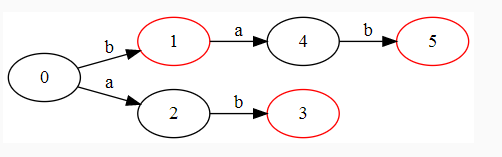
\includegraphics[height=3cm]{g1.png}
    \end{frame}

    \begin{frame}
        \frametitle{介绍}
        这玩意有个非常棒的性质:它包括了 S 的所有子串的信息。\\
        从节点 $0$ 开始,随便走一段必定是 S 的子串,\\
        而 S 的子串也必定是 $0$ 到某一个节点的路径。\\
        并且只要最终走到了红色的节点,这个字符串就一定是原串的一个后缀。\\
        并且,这个「后缀 Trie」是一个 DAG,可以很方便的 dp。\\
        \pause
        唯一也是致命的缺点:这玩意的时空复杂度是 $\mathcal{O}(n^2)$ 的!\\
        看到这里,你应该清楚 SAM 是个什么东西了吧!
    \end{frame}

    \begin{frame}
        没错,SAM 就是一个具有上述性质,并且时空复杂度均为 $\mathcal{O}(n\log\Sigma)$ 的结构!
    \end{frame}

    \section*{概念}

    \begin{frame}
        \frametitle{定义}
        虽说如此,SAM 的概念还是有必要提一句的。  \\
        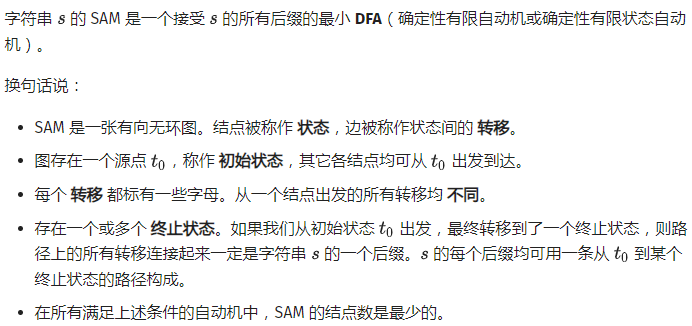
\includegraphics[height=5cm]{g2.png} \\
        From oi-wiki.org

    \end{frame}

    \begin{frame}
        \frametitle{endpos}
        endpos 是什么?\\
        考虑原串 S 的任意非空子串 T,那么\\
        endpos(T) 被定义为 T 在 S 中出现时末尾位置所组成的集合(下标从 1 开始)。\\
        这个可能有点难懂,所以我举个例子:\\
        S = \texttt{"114514"}\textnormal,T=\texttt"14",\\
        那么 endpos(T)=\{3,6\}。\\
        对于空串,我们定义它的 endpos 为 \{0,1,2,3,$\cdots$,|S|\}\\
        是不是非常 Easy?这玩意必须记住,这是重中之重。
    \end{frame}

    \begin{frame}
        \frametitle{endpos}
        我们定义 endpos 等价类为一堆 endpos 相等的子串所组成的集合。\\
        显然,两个不同的 endpos 等价类不可能有相同的元素。\\
        那么这样我们就把一共 $\mathcal{O}(n^2)$ 种子串分成了 $\mathcal{O}(n)$ 种 endpos 等价类。\\
        有人要问了:为啥是 $\mathcal{O}(n)$? 自己翻 OI-wiki 去/xyx
    \end{frame}

    \begin{frame}
        \frametitle{link}
        link,即后缀链接,是 「SAM 上的 fail 指针」。\\
        这玩意很玄学,我们来看看 OI-wiki 的定义吧!\\
        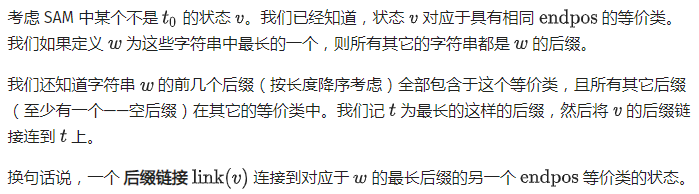
\includegraphics[height=5cm,width=11cm]{g3.png}
    \end{frame}

    \begin{frame}
        \frametitle{link}
        有人会问了:fjy你这样没良心的抄 OI-wiki 好吗?\\
        额……\\
        我们很容易地发现:如果定义一个结点 x 的父节点为 link[x],\\
        那么这就是!一课!树!
        \pause
        恭迎!凸包之神!俞开!!1111
        \pause
        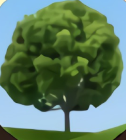
\includegraphics[height=4cm]{g5.png} 
        而根据树的定义,我们似乎也可以把 SAM 叫做 凸包/xyx。
    \end{frame}

    \begin{frame}
        \frametitle{node}
        自动机吗,肯定是有一个个节点组成的。\\
        那么 SAM 的节点是什么呢?\\
        由于有 $\mathcal{O}(n)$ 种 endpos 等价类(下称等价类),\\
        每个 SAM 节点都代表一个等价类内所有的子串的集合!\\
        显然,每个节点代表的 endpos 集合都不同,也就是没有一个字符串同时包含在两个节点里。\\
        当然实现的时候不可能真存一堆字符串,也不会存下 endpos,\\
        否则空间炸出翔。
    \end{frame}

    \begin{frame}
        \frametitle{node}
        那一个 node 里存啥捏?别急,我们先来引入一些记号:\\
        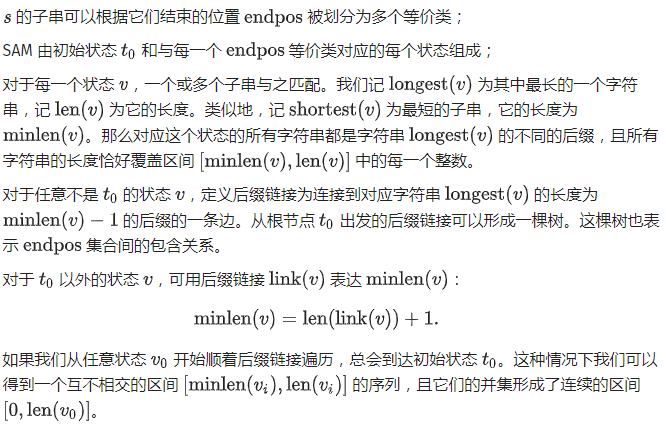
\includegraphics[height=6cm]{g6.png}
    \end{frame}

    \begin{frame}
        \frametitle{node}
        OI-wiki:明天律师函就到你家门口。\\
        谜底揭晓:每个 node 里存 len, link 和 trans。\\
        这个 trans 是啥东西?\\ 
        傻孩子!你自动机连边都不存的吗?
    \end{frame}

    \begin{frame}
        \frametitle{node}
        那问题来了:SAM 中的「边」是怎么定义的呢?\\
        把 endpos 等价类里的所有能拓展的 s 都往后拓展一个字符 c,\\
        这些新字符串所组成的等价类就是这条「边」所指向的节点。\\
        我们来举个例子吧!S=cxyyuyu,节点 \{3,4,6\} 的边 u 所指向节点的 endpos 是什么呢?\\
        \pause
        没错,是 \{5,7\}。\\
        边有两种存法,一种是数组,一种是 std::map\\
        数组的复杂度为 $\mathcal{O}(n)$,但空间为 $\mathcal{O}(n\Sigma)$\\
        std::map 的空间 $\mathcal{O}(n)$,但时间为 $\mathcal{O}(n\log\Sigma)$。\\
        使用时可以自行选择。  
    \end{frame}

    \begin{frame}
        \frametitle{node}
        到了这里,我们总算把定义搞定了。\\
        在看如何实现之前,我们先看几个标准的 SAM。\\
        1. S=cxyuyu,它的 SAM 长这样:\\
        *展示SAM*\\
        很壮观,是不是?
    \end{frame}

    \section{实现}
    
    \begin{frame}
        \frametitle{实现}
        有趣的是,概念似乎比实现还要难/kx\\
        我们先看一下 【模板】,然后边看代码边讲吧。\\
        https://www.luogu.com.cn/problem/P3804
    \end{frame} 

    \section{小结}

    \begin{frame}
        \frametitle{总结}
        SAM 确实是一种比较强大的 string DS。  \\
        它可以很方便地解决很多和后缀有关的东西。\\
        有些本质不同子串问题也可以用它。\\
        总而言之,遇到不会的题,SAM 淦它就对了!\\
        我还会出下一讲——SAM的习题与应用,敬请期待qwq!
    \end{frame}

    \begin{frame}
        \frametitle{Goodbye}
        Thank you for your listening!\\
        Made by fjy666.\\
        参考链接:\\
        https://oi-wiki.org/string/sam/ \\
        https://www.luogu.com.cn/problem/solution/P3804 \\
        https://alpha1022.gitee.io/sam-visualizer/ \\
        https://blog.csdn.net/qq\_42101694/article/details/111740597
    \end{frame}

    \begin{frame}
        \frametitle{Special Thanks}
        Special Thanks to lym(fix \LaTeX\ error in my computer), the oi-wiki and luogu.
    \end{frame}
\end{document}